%%%%%%%%%%%%%%%%%%%%%%%%%%%%%%%%%%%%%%%%%%%%%%%%%%%%%%%%%%%%%%%%%%%%%%%%%%%%%%%%%%%%%%%%%%
%%%  EKAW 2016 - DOREMUS to Schema.org: Mapping a Complex Vocabulary to a Simpler One  %%%
%%%%%%%%%%%%%%%%%%%%%%%%%%%%%%%%%%%%%%%%%%%%%%%%%%%%%%%%%%%%%%%%%%%%%%%%%%%%%%%%%%%%%%%%%%

\documentclass{llncs}

\usepackage{url}
\usepackage{graphicx}
\usepackage{xtab}
\usepackage[inline]{enumitem}
\usepackage[title]{appendix}
\DeclareGraphicsExtensions{.png}


%%%%%%%%%%%%%%%%%%%%%%%%%%%%%%%
%%%  Beginning of document  %%%
%%%%%%%%%%%%%%%%%%%%%%%%%%%%%%%

\begin{document}

\title{DOREMUS to Schema.org: Mapping a Complex Vocabulary to a Simpler One}

\author{Pasquale Lisena\inst{1} \and Rapha\"el Troncy\inst{1}}
\authorrunning{Lisena and Troncy} 
\institute{EURECOM, Sophia Antipolis, France \\
\email{pasquale.lisena|raphael.troncy@eurecom.fr}}

\maketitle

%%%%%%%%%%%%%%%%%%
%%%  Abstract  %%%
%%%%%%%%%%%%%%%%%%

\begin{abstract}
Music metadata are often represented through complex models and ontologies such as FRBRoo. As a consequence, these metadata are not easily consumable by general search engines or external web applications. This paper presents a way for mapping a complex ontology to a simpler model, Schema.org. This methodology is composed of a series of recipes for mapping classes and properties iteratively.

\keywords{Ontology, FRBRoo, Musical Metadata, Schema.org}
\end{abstract}

%%%%%%%%%%%%%%%%%%%%%%%%%
%%%  1. Introduction  %%%
%%%%%%%%%%%%%%%%%%%%%%%%%

\section{Music information and the structured data}
\label{sec:introduction}

Users are nowadays used to see an enrichment in the results of search engines. This is made possible thanks to the adoption of some form of \textit{Structured Data markup}, like Schema.org \cite{guha2015schema} that allows to describe contents on the page in a machine-understandable way. In particular it offers classes like CreativeWork, Event and music-specific subclasses like MusicComposition or MusicEvent.

Musical works are complex objects that requires complex ontologies for expressing their rich information. FRBRoo is an ontology for describing bibliographic information \cite{doerr2008frbroo}. The central feature of the ontology is the presence of the triplet of classes Work Event-Expression: every artistic Work, only exists through an Event of creation, that realizes the Work itself into an Expression.The DOREMUS ontology\footnote{\url{http://www.doremus.org}} \cite{achichidoremus} extends FRBRoo with music-specific classes and properties like the key, the genre, the casting. Because of this complexity, the consumption of these ontologies by search engines and external applications is not easy.
Nogales et al. \cite{nogales2016linking} performed a mapping between classes and properties in Schema.org and different vocabularies which have exactly the same name (or synonyms).
Godby \cite{godby2013relationship} proposes to map each level of the chain Work - Expression - Manifestation - Item with a entity of the CreativeWork class, a limit of this strategy is that the information is split up among different objects.

In this paper, we provide a strategy for translating a complex ontology like DOREMUS into Schema.org, structured as a series of recipes to follow.
This method is based on the observation of the graph and it assumes sufficient knowledge of the involved models. As example, we will try to represent Beethoven's \textit{Sonata ``Quasi una Fantasia"}, described in DOREMUS (``mus", later) in Figure \ref{fig:beet-doremus}, using Schema.org (``sdo").

\begin{figure}
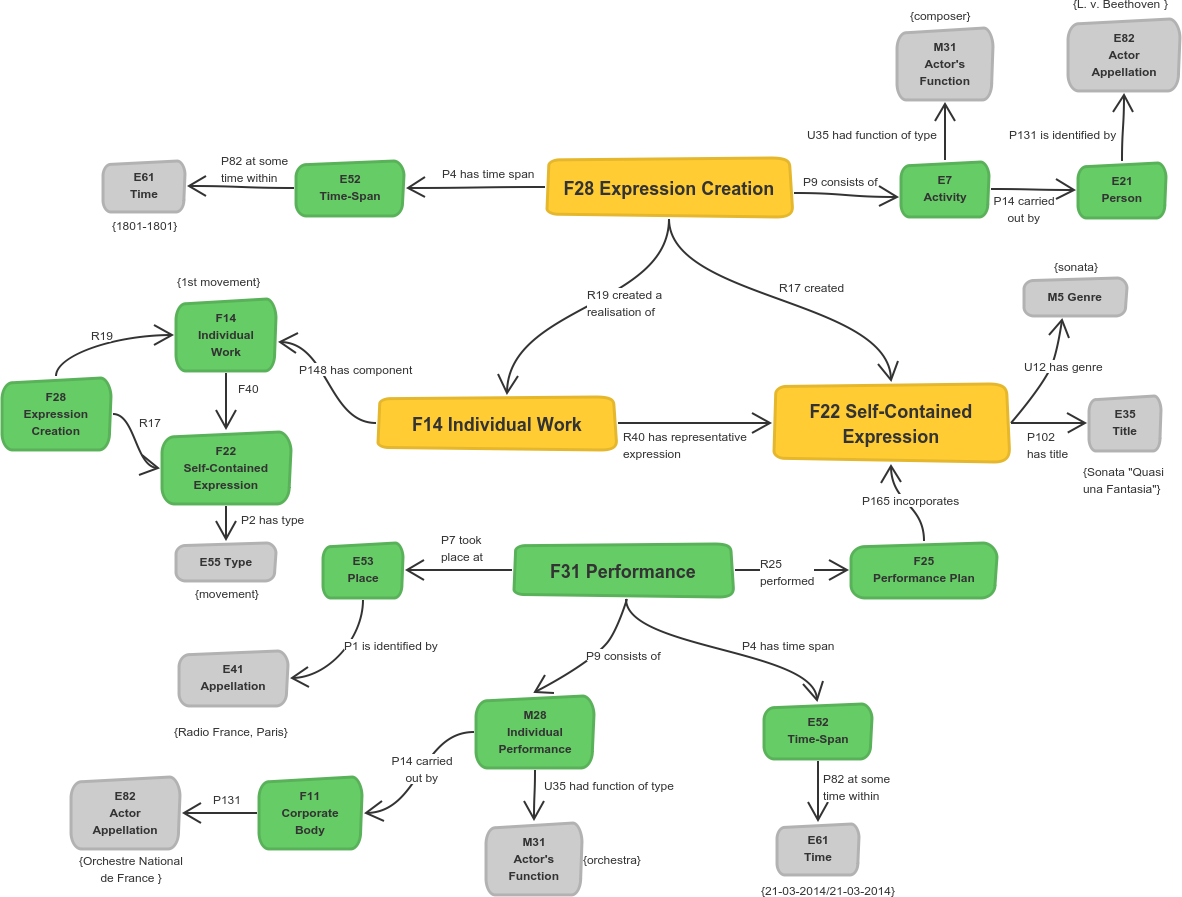
\includegraphics[width=11cm]{img/Beethoven-Doremus.png}
\centering
\caption{Graph of Beethoven's \textit{Sonata ``Quasi una Fantasia"} in DOREMUS.}
\label{fig:beet-doremus}
\end{figure}


%%%%%%%%%%%%%%%%%%%%%%%%%%%%%%%%%
%%%  3. Model simplification  %%%
%%%%%%%%%%%%%%%%%%%%%%%%%%%%%%%%%

\section{Model simplification}
\label{sec:simplification}

\subsubsection{Choose the starting node.}
The most suitable starting point should coincide with the most significant class or classes in the starting ontology, DOREMUS. It could be the class with the highest number of occurrences, or it could consist in a frequent pattern, like the FRBRoo triangle. We choose as starting node \textit{mus:F2 Expression} and \textit{mus:F28 Expression Creation}, because they are linked with most of the crucial information for the final user, the title and the composer.

\subsubsection{Identify similar classes.}
\label{sec:classmap}
For each class in DOREMUS, the best match in Schema.org should satisfy one or more of these criteria:
\begin{enumerate*}
 \item{
They should have similar names, where similarity is computed using the Levenshtein distance or the number of common synonyms.
}
 \item{They should have similar descriptions, where the similarity can be computed through the Cosine or the Token-Wise distance.}
 \item{They should have similar properties}
 \item{They should have similar expected property values.
e.g. both \textit{mus:U12 has genre} and \textit{sdo:musicCompositionForm} have ``sonata" as possible value.
}
\end{enumerate*}

If the research for a suitable match fails for a specific class, then it could mean that Schema.org does not describe it. In this case, you can decide if that information is too specific and does not need to be mapped or that it is possible represent it as plain text in a note. Alternatively, you  can consider it as a candidate for an extension of Schema.org.

\subsubsection{Identify similar properties.}
For each class mapped, we must map its properties. The criteria are:
\begin{enumerate*}
 \item{They should have similar name.}
 \item{They should have similar description.}
 \item{They should have similar expected value.}
\end{enumerate*}

Each mapped property could have as value a literal (e.g. key and genre) or another class  (e.g. the composer is a Person). In the latter case, if we have not previously mapped this class, we consider it as a new input for the first steps, until every node in the graph is reached.

\subsubsection{Simplify the graph.}

It could happen that the same type in Schema.org map is mapping multiple DOREMUS classes: i.e. \textit{sdo:MusicComposition} results to map both Works and Expressions. Merging these nodes can produce the advantage of a simpler model, in which the information is distributed in as less nodes as possible. Two nodes are good candidates for the merging when:
\begin{enumerate*}
\item{They have the class or a superclass in common.}
\item{The direct connections with the same class are realized with the same properties.}
\item{They are directly connected between them.}
\item{They have not conflicting properties.}
\end{enumerate*} The \textit{mus:F1 Work} and \textit{mus:F2 Expression}, both mapped with \textit{sdo:Music-Composition}, satisfy all these criteria. Moreover, the difference between Work and Expression is slight since from the FRBRoo and it has been considered not relevant from the point of view of Schema.org \cite{godby2013relationship}.

Redundant nodes are substituted with a new node with:
\begin{enumerate*}
\item{The same class of the original ones (or the most specific among the two)}
\item{The sum of their properties.}
\end{enumerate*}
The result of this phase is a new graph as it is show in Figure \ref{fig:beet-schema}.

\begin{figure}
\centering
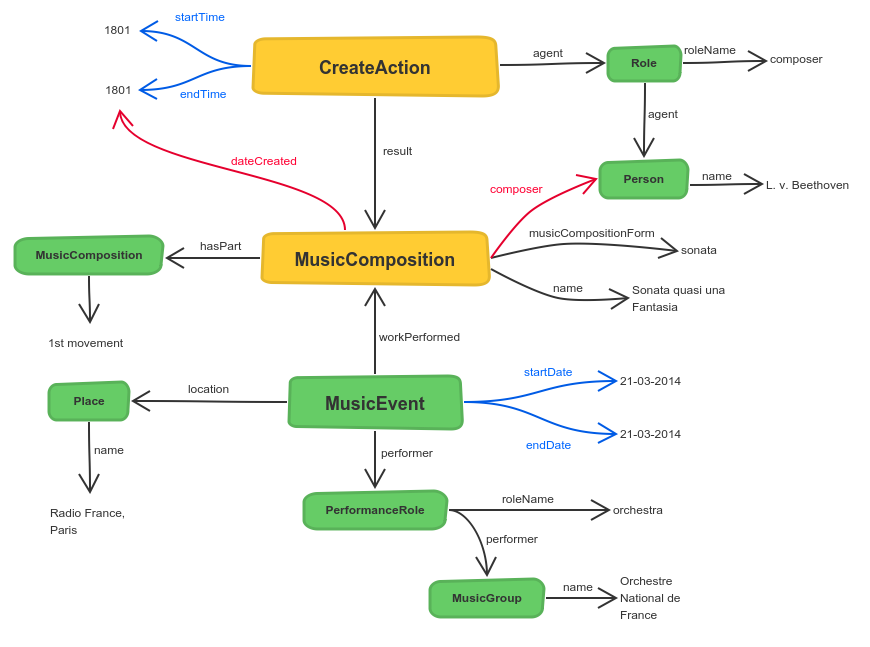
\includegraphics[width=11cm]{img/Beethoven-Schema.png}
\caption{Graph of Beethoven's \textit{Sonata ``Quasi una Fantasia''} in Schema.org.}
\label{fig:beet-schema}
\end{figure}


%%%%%%%%%%%%%%%%%%%%%%%%
%%%  4. Evaluation   %%%
%%%%%%%%%%%%%%%%%%%%%%%%

\section{Evaluation and Future Work}
\label{sec:evaluation}

The evaluation of the goodness of the mapping is a long term goal, that can be performed only when data will be more easily consumed (e.g. by search engines). For having a quick feedback on it, we prepared a JSON-LD version of the \textit{Sonata Quasi Una Fantasia} available at \url{https://db.tt/em0GxWbT}.
Both the Structured Data Testing Tool by Google\footnote{\url{https://search.google.com/structured-data/testing-tool}} and the Structured Data Linter\footnote{\url{http://linter.structured-data.org/}} show the structure of the Schema.org graph like a tree, with 76 statements correctly recognized. The Structured Data Linter offers in addition a preview of the result as they could be shown in a SERP.
For having a stronger visual feedback, we developed a lightweight web app, named Schema.org Visualizer\footnote{\url{https://github.com/pasqLisena/schema-visualizer}}, which consumes the data in JSON-LD and shows a knowledge cards for the described contents. The result for our example is available at \url{https://goo.gl/mCAszw}.

We are planning to test our recipes on the ELI ontology\footnote{\url{http://publications.europa.eu/mdr/eli/}}. The goal is comparing the result of the mapping to the one which has recently been handmade performed\footnote{\url{https://github.com/schemaorg/schemaorg/issues/1156}}.

Future works will include an implementation strategy for this methodology, that will also highlight the contents excluded from the mapping, in order to better evaluate the possibility of presenting a Schema.org extension.

%%%%%%%%%%%%%%%%%%%%%%%%%%%%%%%%%%%%%%%
%%%  5. Conclusion and Future Work  %%%
%%%%%%%%%%%%%%%%%%%%%%%%%%%%%%%%%%%%%%%

%\section{Future Work}
%\label{sec:conclusion}

%We plan an exhaustive evaluation of our approach by using the recipes widely in DOREMUS and in different ontologies. A further subject of study is the generation of an algorithm that, starting from the recipes, identifies the best candidates for mapping, as well as classes and properties that are excluded in this process, often because they have not correspondence in Schema.org ontology (i.e. the librarian cataloging, the desired casting, the tempo). We are evaluating the possibility of proposing a musical extension for Schema.org or for the \textit{bib.schema.org} extension.

%The result of the mapping described in this paper will be soon integrated in a web application for the exploration of musical data, realized in the context of the DOREMUS project.

\subsubsection*{Acknowledgments.}
This work has been partially supported by the French National Research Agency (ANR) within the DOREMUS Project, under grant number ANR-14-CE24-0020.

% ---- Bibliography ----
\bibliographystyle{abbrv}
\bibliography{bib-doremus}

\newpage

\end{document}